\documentclass{standalone}
\usepackage{tikz}
\usepackage{pgfplots}
\usetikzlibrary{positioning,3d,decorations.markings,calc}
\pgfplotsset{compat=1.18}

\begin{document}
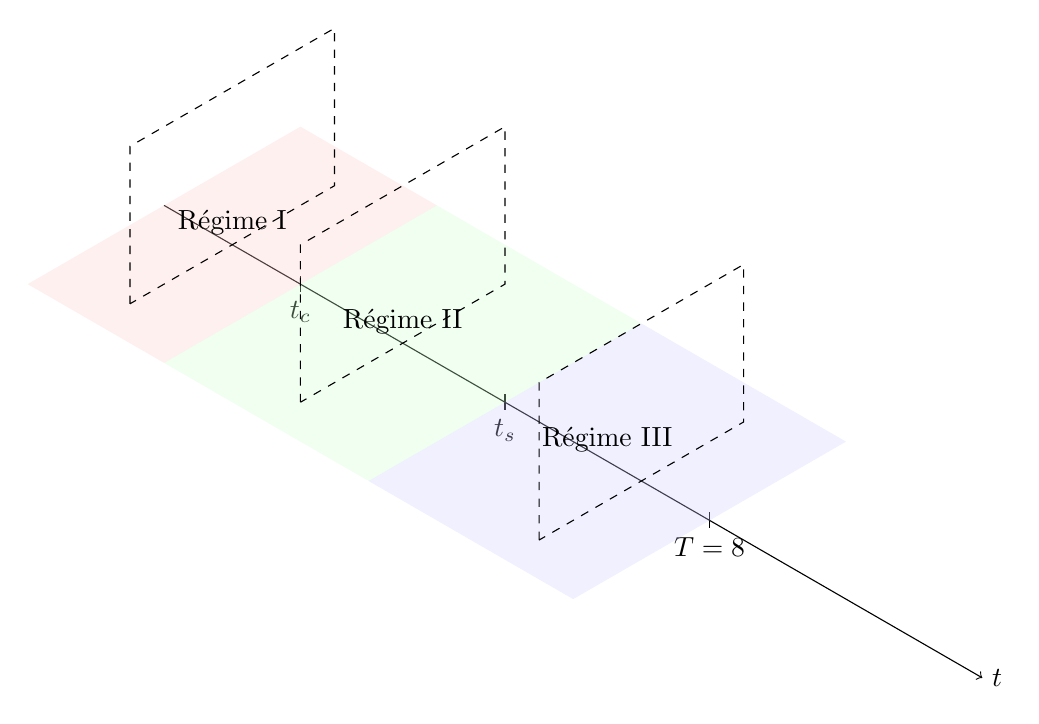
\begin{tikzpicture}[
    x={(0.866cm,-0.5cm)},
    y={(0.866cm,0.5cm)},
    z={(0cm,1cm)}
]
    % Axe temporel
    \draw[->] (0,0,0) -- (12,0,0) node[right] {$t$};
    
    % Points temporels importants
    \draw (8,0,0.1) -- (8,0,-0.1) node[below] {$T=8$};
    \draw (5,0,0.1) -- (5,0,-0.1) node[below] {$t_s$};
    \draw (2,0,0.1) -- (2,0,-0.1) node[below] {$t_c$};
    
    % Zones de régimes colorées
    \fill[blue!20,opacity=0.3] (8,-2,0) -- (8,2,0) -- (5,2,0) -- (5,-2,0) -- cycle; % Régime III
    \fill[green!20,opacity=0.3] (5,-2,0) -- (5,2,0) -- (2,2,0) -- (2,-2,0) -- cycle; % Régime II
    \fill[red!20,opacity=0.3] (2,-2,0) -- (2,2,0) -- (0,2,0) -- (0,-2,0) -- cycle; % Régime I
    
    % Labels des régimes
    \node[above] at (6.5,0,0) {Régime III};
    \node[above] at (3.5,0,0) {Régime II};
    \node[above] at (1,0,0) {Régime I};

    % Encarts pour les coupes (y,z) - maintenant perpendiculaires à l'axe du temps
    \draw[dashed] (1,-1.5,0) -- (1,-1.5,2) -- (1,1.5,2) -- (1,1.5,0) -- cycle; % Encart Régime I
    \draw[dashed] (3.5,-1.5,0) -- (3.5,-1.5,2) -- (3.5,1.5,2) -- (3.5,1.5,0) -- cycle; % Encart Régime II
    \draw[dashed] (7,-1.5,0) -- (7,-1.5,2) -- (7,1.5,2) -- (7,1.5,0) -- cycle; % Encart Régime III

\end{tikzpicture}
\end{document}
